\documentclass[10pt,a4paper,twoside]{article}
\usepackage[dutch]{babel}
%laad de pakketten nodig om wiskunde weer te geven :
\usepackage{amsmath,amssymb,amsfonts,textcomp}
%laad de pakketten voor figuren :
\usepackage{graphicx}
\usepackage{float,flafter}
\usepackage{hyperref}
\usepackage{inputenc}
%zet de bladspiegel :
\setlength\paperwidth{20.999cm}\setlength\paperheight{29.699cm}\setlength\voffset{-1in}\setlength\hoffset{-1in}\setlength\topmargin{1.499cm}\setlength\headheight{12pt}\setlength\headsep{0cm}\setlength\footskip{1.131cm}\setlength\textheight{25cm}\setlength\oddsidemargin{2.499cm}\setlength\textwidth{15.999cm}

\begin{document}
\begin{center}
\hrule

\vspace{.4cm}
{\bf {\Huge Problem 4}}
\vspace{.2cm}
\end{center}
{\bf Name: Cheng Chen}  \\
{\bf ID:40222770}\\
{\bf function: tan(x)}\\
{\bf Concordia University}\\
SOEN 6011: Software Engineering Processes {\bf  } \hspace{\fill}  17 July  2022 \\
\hrule
%\bf genereert vette letters, \large \Large \huge \Huge \tiny \small ... verschillende lettergroottes, met \em, \it, \sl krijg je cursieve tekst
%Je moet accolades gebruiken om aan te geven waarop je het commando precies wil laten inwerken.
% commentaar zet je in de tex-file met een %-tekentje voor.



%de ~ zorgt ervoor dat het ! met een spatie aan de tekst wordt geplakt en niet naar de volgende lijn verhuist.  Omdat latex na elk . automatisch een dubbele spatie invoegt, kan je ~ ook gebruiken om te voorkomen dat je na een afkorting bvb.~een dubbele spatie krijgt.

%1 open lijn wordt door latex gewoon als spatie gezien, met twee linefeeds  begint een nieuwe paragraaf.  Als je wil voorkomen dat de tekst inspringt, kan je het commando \noindent gebruiken.  \\ springt naar een volgende lijn, \newpage naar een volgend blad.


%\begin{figure}
%\centering
%\includegraphics[width=0.7\linewidth]{figje}
%\caption{}
%\label{fig:figje}
%\end{figure}
\section{Description}
\subsection{Debugger}
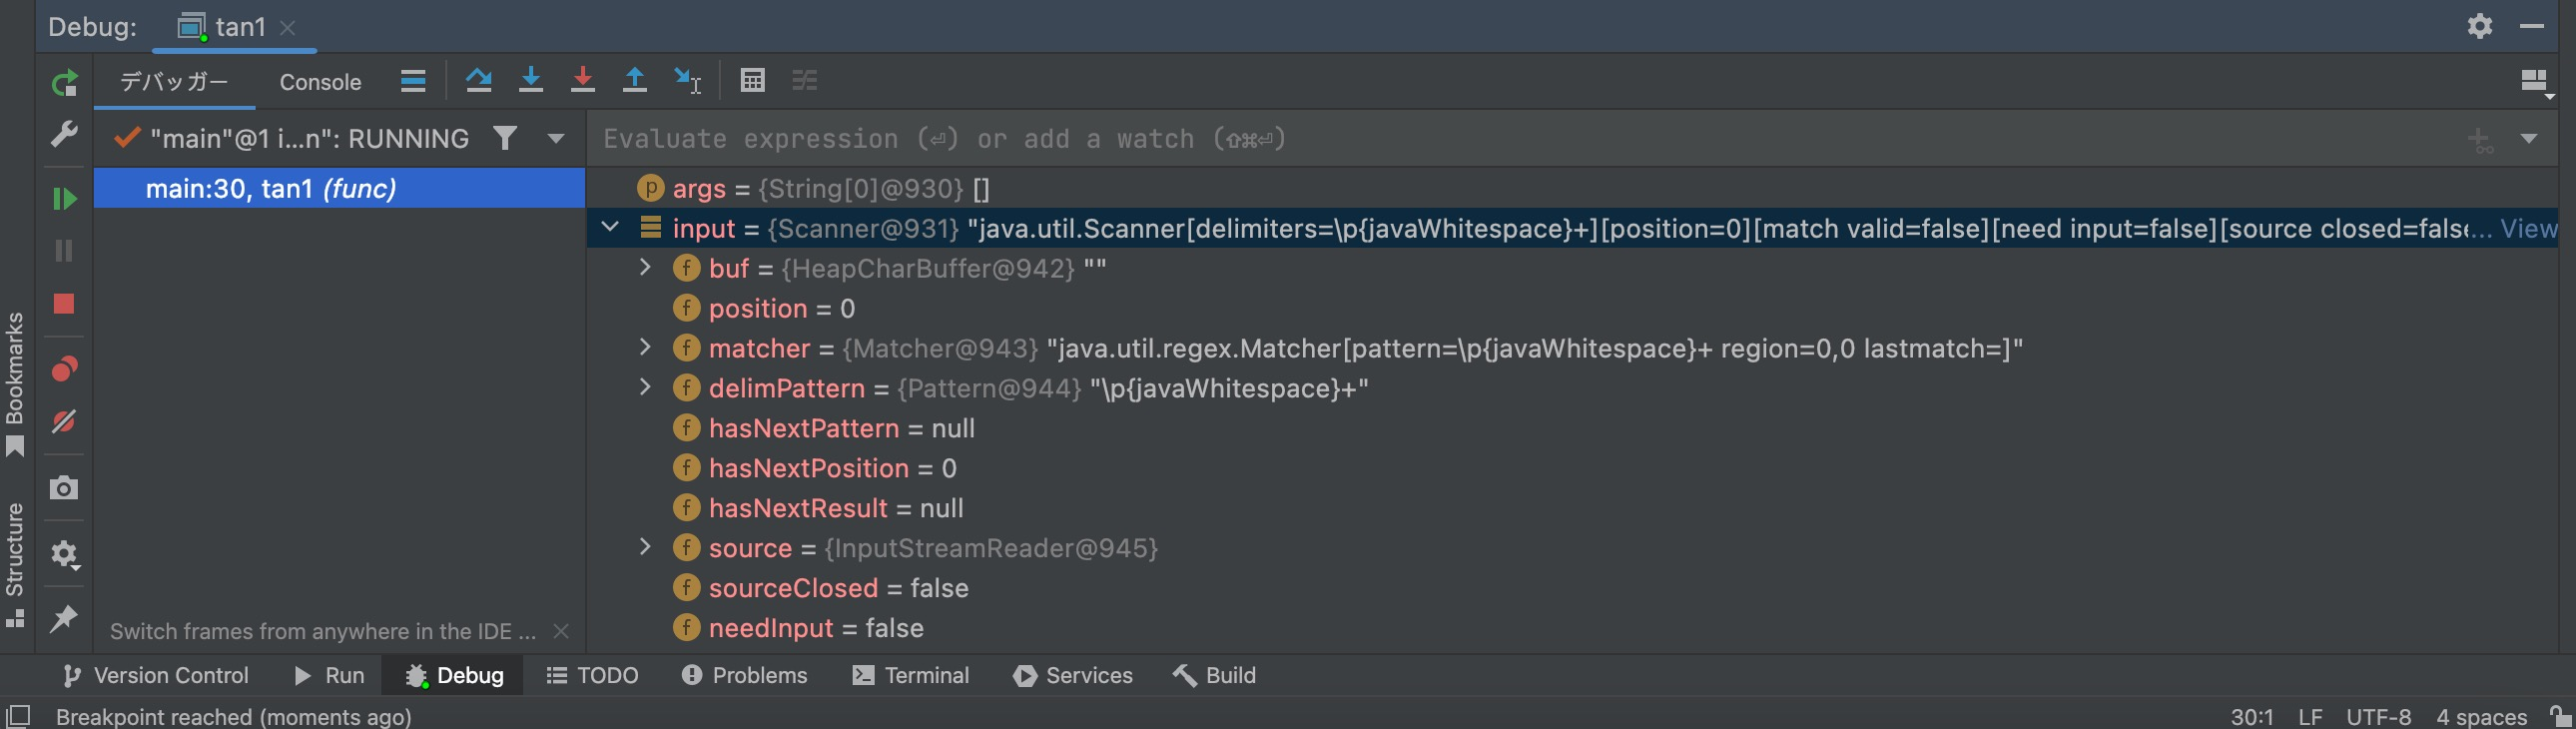
\includegraphics[scale=0.15]{debugger.png}
\subsection{Mindmap}
\includegraphics[scale=0.24]{TooLTT.png}
\item 
Advantages: report error immediately.
\item
Disadvantages:hard to help if the execution is stopped inside an invariant.
\subsection{code characteristics}
correct:99 percent accuracy.
robust:check if the input is right.
time-efficient:use a hard-coded formula.
usable:can compute tan(x) with 0.01
%Met het commando \sectie{naamtitel} maak je een nieuwe titel aan.

\section{Checkstyle}
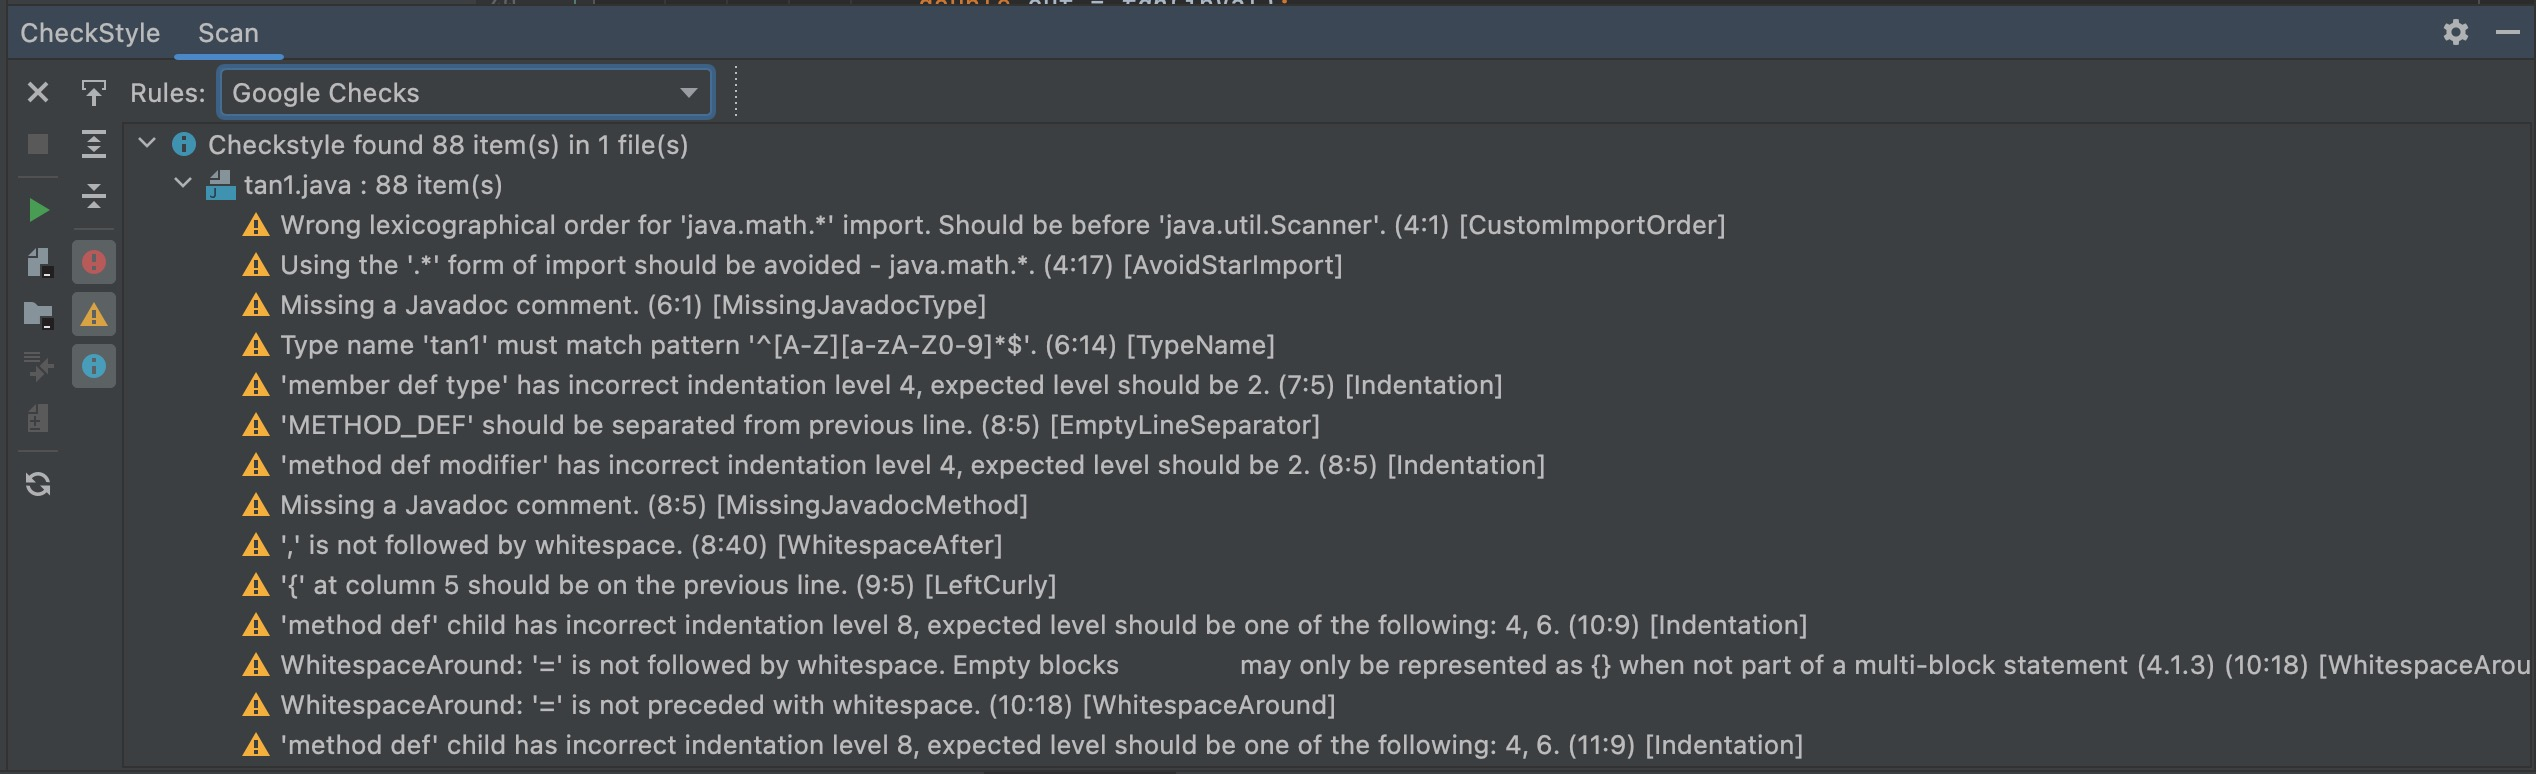
\includegraphics[scale=0.15]{Checkstyle.png}
\item
description: Checkstyle snapshot of my tan(x) function source code.
\item
advantages:Some information are good for making my source code more easily readable.
\item
disadvantages:Some information are not necessary.


%hier werd verwezen naar de tabel die als \label (naam} 'tabel1' kreeg.


%met enumerate genereer je een opsomming, itemize maakt verschillende puntjes

\end{document}
